\documentclass{article}

% Language setting
% Replace `english' with e.g. `spanish' to change the document language
\usepackage[utf8]{inputenc}
\usepackage[T1]{fontenc}
\usepackage[english]{babel}
\usepackage{authblk}        % gestion auteurs/affiliations
% Set page size and margins
% Replace `letterpaper' with `a4paper' for UK/EU standard size
\usepackage[letterpaper,top=2cm,bottom=2cm,left=3cm,right=3cm,marginparwidth=1.75cm]{geometry}

%\usepackage[left, modulo]{lineno}
%\linenumbers

% Useful packages
\usepackage{tabularx}
\usepackage{array}
\renewcommand{\arraystretch}{1.3}
\usepackage{rotating}
\usepackage{amsmath}
\usepackage{graphicx}
\usepackage[colorlinks=true, allcolors=blue]{hyperref}
\usepackage{csquotes} % très recommandé avec biblatex
\usepackage[backend=biber,style=authoryear]{biblatex} 
\addbibresource{ifall_bordeau.bib} % nom de ton fichier .bib

\title{Lost in Navigation? Ensuring Living Lab Frameworks Stay on Course with Local Needs}
%\title{De l'anthologie de l'absurde à la symphonie locale : trajectoire d'un projet qui a touché terre}
% Auteurs (indices entre crochets = affiliations)
\author[6,5]{E. Delay\thanks{etienne.delay@cirad.fr}}
\author[1]{A.Hertzog-Adamczewski}
\author[3,4]{R. Duboz} % email en note
\author[1,2]{A. Ogilvie}
\author[5]{W. Daré}
\author[6]{A. Bah}
\author[7]{O. Samaké}

% Affiliations
\affil[1]{CIRAD, UMR G-EAU, F-34398 Montpellier, France.}
\affil[2]{IRD, UMR G-EAU, F-34398 Montpellier, France.}
\affil[3]{CIRAD, UMR ASTRE, F-34398 Montpellier, France.}
\affil[4]{IRD, UMI UMMISCO, Hann Mariste, Dakar, Sénégal}
\affil[5]{CIRAD, UMR SENS, F-34398 Montpellier, France.}
\affil[6]{CIRAD, UMR SENS, Ecole Superieur polytechnique de Dakar, UCAD, Sénégal}
\affil[6]{SAED, Saint-Louis, Sénégal}

\begin{document}
\maketitle
\begin{abstract}
Participatory modeling approaches, particularly those rooted in Companion Modeling (ComMod), are often credited with initiating socio-environmental transformations. Examples from Zimbabwe \parencite{perrotton_my_2017} and Burkina Faso \parencite{dare_dynamique_2016} illustrate how these methods have facilitated engagement between stakeholders, sometimes leading to institutional changes over extended periods. However, the effectiveness of such approaches is contingent on their alignment with local realities and pressing challenges. The question remains: who holds the compass in these participatory frameworks? Do researchers, institutions and players succeed in abandoning their agenda? A case study from the Lake Guiers region in Senegal highlights the tensions between knowledge production, local agency, and transformative action.

After several years of engagement with local communities through participatory workshops, a pivotal moment occurred in different arena : when a doctoral student presented her findings on hazardous chemical pollutants in the lake's water, when allochtone populations spoke out against their refusal to respect fishing restrictions face to face with native fishermen (Delay et al. 2023).  Unlike previous discussions on ecosystem management, which were perceived as peripheral to daily survival, this revelation directly impacted livelihoods, exposing communities to immediate and invisible risks. The local response—calls for awareness campaigns and regulatory interventions—raised deeper questions about the adequacy of conventional participatory approaches. How can living lab models move beyond knowledge dissemination towards tangible systemic transformation? How can scientific findings generate experiential urgency rather than passive information?

Recent scholarship suggests that for knowledge to trigger action, it must engage stakeholders not just intellectually/abstract, but affectively — a concept referred to as "affective knowing" \parencite{hertz_knowledge_2025}. This perspective challenges traditional scientific detachment and underscores the need for transformative science that actively catalyzes change rather than merely observing it. A more reflexive and adaptive governance model is necessary—one that situates knowledge within local dispositifs (assemblages of discourses, institutions, and power structures). Rather than assuming that participatory models inherently lead to transformation, they must be reconfigured to align with the strategic urgencies of a given territory. This shift demands a reconsideration of the role of scientists in participatory governance: are they facilitators, guides, or interveners? By embedding participatory models within affective and political landscapes, living labs in Senegal and beyond can become true engines of systemic change rather than passive spaces for stakeholder dialogue.
\end{abstract}

\section{Introduction}

The future is radically uncertain. Accordingly, actors orient their decisions based on imaginaries and narratives often supported by computational technologies (models, algorithms, forecasting devices). \textcite{beckert_uncertain_2018} propose the notion of “fictional expectations” (rather than “rational” ones): these socially shared fictions coordinate action and exert performative effects.  

From its inception, the \textit{\textit{Santés \& Territoires}} project sought to embrace an approach that integrates the imaginaries of local populations and of the researchers engaged in the project’s study areas, in order to account for the imaginaries carried by each stakeholder. The objective of the \textit{\textit{Santés \& Territoires}} project\footnote{santes-territoires.org} (2021–2026) is to support agroecological transitions within a \textit{One Health} framework through the establishment of \textit{Living Labs}. According to the \textit{One Health High-Level Expert Panel (OHHLEP)}, \textit{One Health} is an integrated health approach aimed at sustainably balancing and optimizing the health of people, animals, and ecosystems. \textit{One Health} recognizes that the health of humans, domestic and wild animals, plants, and the environment as a whole are closely interconnected and interdependent\footnote{https://www.who.int/groups/one-health-high-level-expert-panel, accessed August 21, 2025}. Consequently, \textit{One Health} is an interdisciplinary and multisectoral approach. Initially, \textit{One Health} was primarily advanced by veterinary and public health fields, focusing on human diseases of animal origin (zoonoses). Since the United Nations Environment Programme (UNEP) joined the quadripartite agreement in 2022 with the World Health Organization (WHO), the World Organisation for Animal Health (WOAH), and the Food and Agriculture Organization (FAO), the applications of the \textit{One Health} concept have struggled to effectively incorporate ecological and agricultural dimensions, even though these domains play a central role in human and environmental health. To address this gap, the \textit{\textit{Santés \& Territoires}} project operationalizes the \textit{One Health} approach within the framework of socio-ecological system health as defined by \textcite{de_garine-wichatitsky_health_2021}, and draws on a systemic and participatory health perspective \parencite{duboz_systems_2018}. The integration of participatory engineering and socio-ecological systems provides tools, methods, and a genuinely transdisciplinary theoretical framework to facilitate science–society dialogue.  

For \textcite{pfotenhauer_learning_2012}, technical and social approaches cannot be separated. Real-world objects are deeply intertwined with the lives of those who use and live around them. It is therefore necessary to involve populations and policymakers in decision-making.  

Our methodological approach builds on a longitudinal observation of the \textit{\textit{Santés \& Territoires}} project in Senegal, through the analysis of grey literature produced by project members and archived on a shared platform, complemented by our field notes. The objective is to identify sequences—what \textcite{jasanoff_constitutional_2011} calls “constitutional moments”—in which affect intervenes in the emergence or reconfiguration of an arrangement. These are situations in which established representational frameworks no longer suffice, and new meanings—whether identity-based, memorial, or related to belonging—transform relationships and reshape the arrangement \parencite{hertz_knowledge_2025}. Such moments serve as analytical windows where dominant imaginaries are contested and realigned.  

Our reinterpretation of the project’s events is guided by two conceptual axes: \textit{(i)} the goal of stakeholder empowerment, supported by the “charter of accompaniment” defined by the ComMod collective \parencite{barreteau_our_2003} and set as a prerequisite for project action, and \textit{(ii)} \textit{One Health} as a unifying thread that (as we will see) helps maintain, as much as possible, a shared value alignment among project participants. Yet, echoing \textcite[p.144]{beck_governance_2021} on the notion of \textit{sustainability}, we observe that behind the collective commitment to working within a \textit{One Health} framework persist sectoral differences, sustained by value conflicts, divergent imaginaries, and intercultural variations in research practices—all of which hinder value alignment.  

The \textit{Santés \& Territoires} project thus examines the links between ways of representing and knowing phenomena, on the one hand, and ways of acting upon them to foster transformation, on the other. This is, ultimately, the core ambition: to accompany transformations in cultural and practical domains with a view to improving the overall health of socio-ecological systems.  

In this paper, we therefore take up the question posed by \textcite[p.148]{beck_governance_2021}: “\textit{how citizenship gets imagined and enacted; who gets to participate and who is entitled to speak for sustainable futures, as well as who does not belong and hence lacks such voice?}” We do so by focusing on the operational reconfigurations at work within the dynamics of the project’s \textit{Living Labs} in Senegal. 


\section{Materials and Methods}
\subsection{Theoretical Framework: The Assemblage Approach}

The theoretical framework mobilized in this article draws on the assemblage approach, often associated with Actor–Network Theory \parencite{callon_techno-economic_1990, goulet_characterizing_2021}, to which \textcite{hertz_knowledge_2025} add the dimension of affect. An assemblage can thus be defined as a dynamic configuration that brings together heterogeneous elements—human and non-human, material and immaterial, discursive and practical. The notion of assemblage partly overlaps with the concept of \textit{dispositif} proposed by \textcite{foucault_jeu_1977}. According to \textcite{hertz_knowledge_2025}, the specificity of assemblages lies in their capacity to generate a powerful shared experience, which the authors call \textit{affect}: an experiential intensity capable of triggering concrete, situated actions. This perspective makes it possible to move beyond a purely representational or abstract conception of knowledge, by fully integrating the sensitive and relational dimensions of collectively produced knowledge.  

Affect here refers to the idea that genuinely operative knowledge cannot be reduced to abstract discursive content: it must be felt and experienced in order to produce real effects on the actors involved. The assemblage approach thus emphasizes that it is through encounters and interactions between bodies, practices, discourses, and sensibilities that knowledge acquires its transformative potential \parencite{bessy_experts_1995}. In the same vein, the works of \textcite{jasanoff_constitutional_2011, beck_governance_2021} mobilize the notion of affect in their call to summon imaginaries that can shift windows of opportunity in innovation.  

Alignment corresponds to the progressive and often unpredictable articulation of elements that are initially dispersed or in tension. This process generally requires a favorable relational context, one that fosters mutual recognition of the knowledge mobilized by actors with diverse representations \parencite{geels_typology_2007}. \textcite{jasanoff_constitutional_2011, hertz_knowledge_2025} emphasize in particular the importance of concrete and situated moments—such as participatory activities or shared experiences—that allow the various elements of the assemblage to gradually converge and produce a shared world \parencite{arendt_condition_1957}.  

Finally, the assemblage approach calls for a renewed reflexive posture for researchers and practitioners engaged in co-production processes. They are invited to become “managers of meaning” rather than mere producers or transmitters of knowledge. Their role consists in facilitating conditions conducive to the emergence of shared affects, capable of durably federating actors around a common knowledge–action. This shift in posture also implies valuing flexible methods, open to contingency and attentive to the affective dynamics that traverse all collective knowledge-production processes.  

\subsection{Chronological Evolution of the Living Labs in Senegal}

The first phase, devoted to diagnosis, occupied the initial year of the project. It enabled the mapping of localities and arenas of actors where the Living Labs—these fragile spaces of experimentation—would take root. Two Living Labs were initiated around Lake Guiers: one in the commune of Mbane and the other in the commune of Keur Momar Sarr (see Section~\ref{sec:Phaseinit}).  

In these sites, researchers identified issues that were not simply “problems” in the institutional sense, but points of attachment—lines of flight—around which interdisciplinary thematic groups began to form. The ambition was not to reproduce the weight of institutional frameworks, but rather to co-invent, together with residents, questions that take root locally, grounded in what endures despite everything. This unfolded mainly during the second year (see Sec.~\ref{sec:phaseIntermediaire}), when participants in each location slowly began to enter the process. Their integration depended less on their availability than on the facilitators’ ability to adopt a different posture: relinquishing the role of pilots in order to risk the uncertainties of co-accompaniment.  

From the third year onward, activities rooted in the materiality of place deepened. They began weaving threads of unforeseen interactions, generating synergies that no one had anticipated (see Sec.~\ref{sec:phaseAgencements}). Certain initiatives, carried by dispersed groups, suddenly resonated elsewhere—a fragile echo, but sufficient for worlds to recognize and align with one another.  

Each year, the scientists gathered in an annual assembly—a moment when hypotheses were still exchanged in germinal form, and results remained tentative, in the process of sedimentation.  

Starting in the second year, additional arenas opened up: the \textit{Kourel}, forums organized in the villages. These spaces of dialogue and negotiation made it possible to discuss ongoing activities and to reorient investigations. Gradually, the \textit{Kourel} gained importance, shifting the project’s center of gravity. Within these fragile arenas, where uncertainty was shared, resided a discreet hope: that by the time the project concludes, in two years’ time, the participants in these “constitutional events” will be able to directly engage the worlds of research and development, carrying the voices of those most directly concerned—the inhabitants.  

\subsection{Documentation \textit{in itinere}}

The project succeeded in establishing a practice still relatively uncommon in action-research initiatives in the Global South: the systematic uploading of heterogeneous documents produced during the project onto a shared storage space. After three years of work in Senegal, the project’s researchers (more than fifty in total) had produced and pooled no fewer than 2,437 documents (jpg, pdf, docx, etc.) related to Senegal (see Fig.~\ref{fig:filetype}).  

\begin{figure}
    \centering
    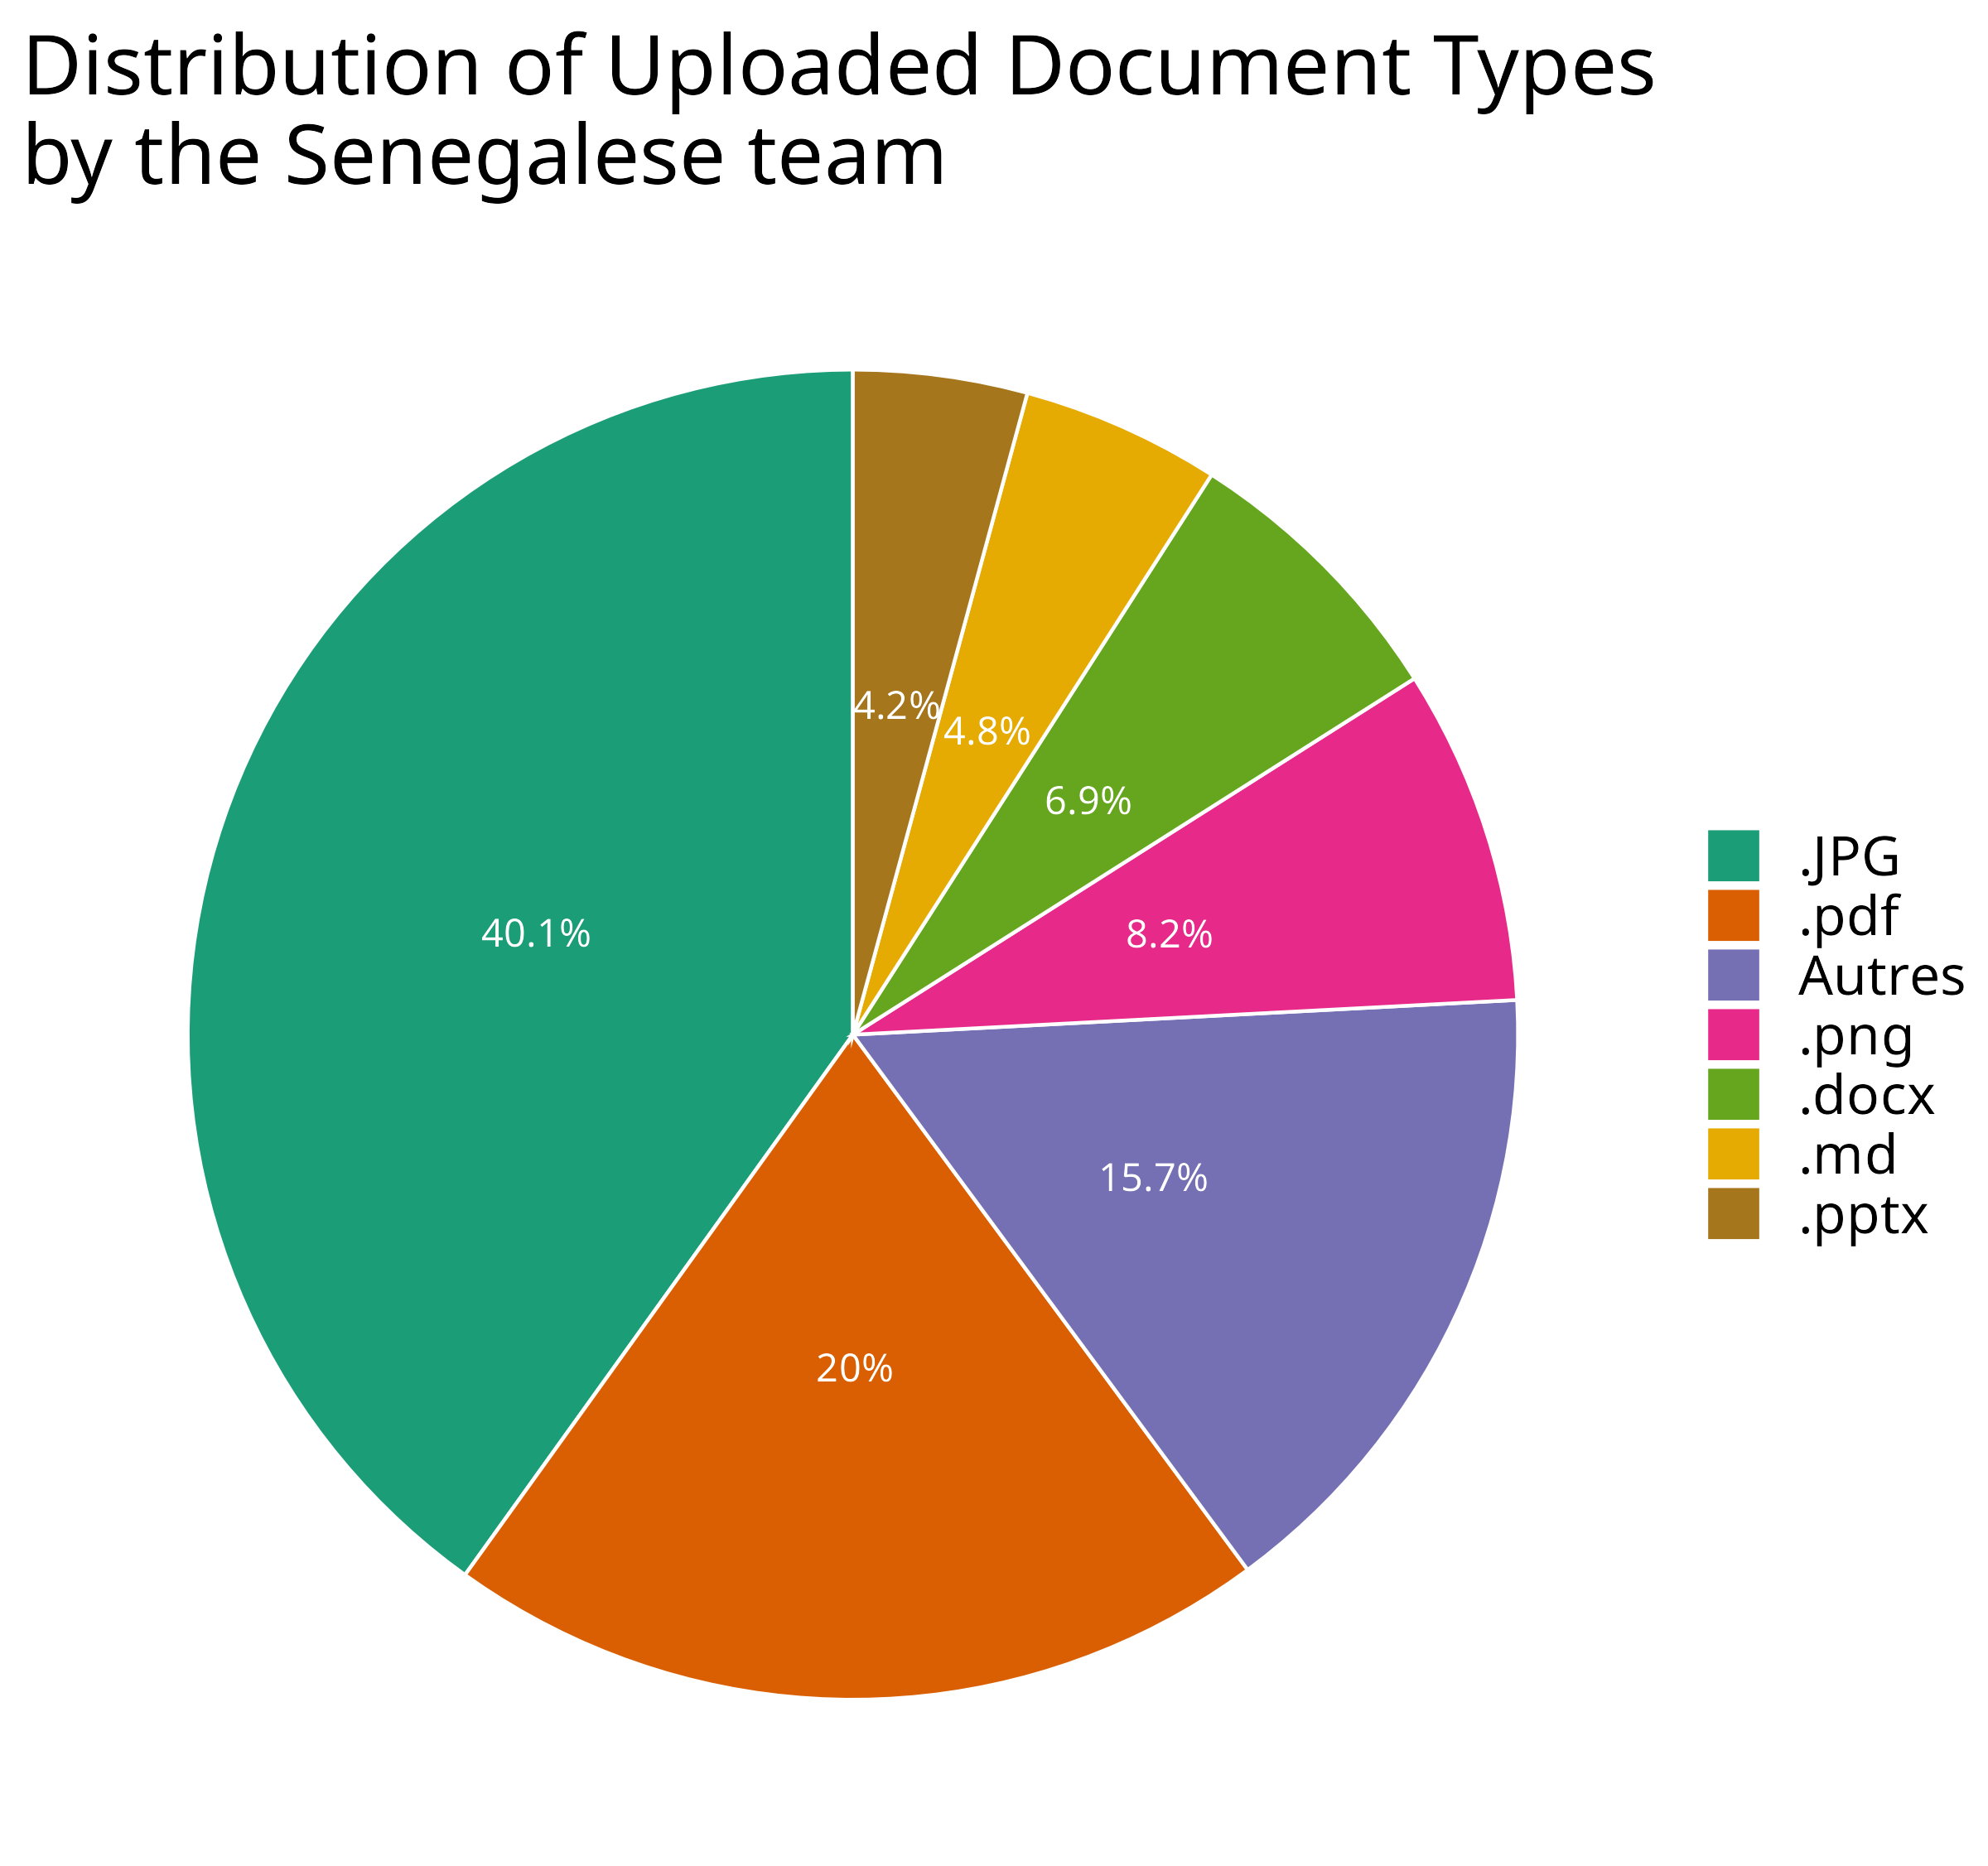
\includegraphics[width=0.6\linewidth]{img/doc_proportion.png}
    \caption{Proportion of different types of documents stored in the project’s “Senegal” cloud space. Of the 9GB of data stored, 35 file types were identified. Among these, the seven categories shown here each represent more than 4\% of the data. Images account for 48\% of documents (jpg+png), while textual documents represent 35\% (pdf+docx+md+pptx).}
    \label{fig:filetype}
\end{figure}

This illustrates that primary research data are relatively underrepresented, whereas synthesized documents are systematically uploaded. In our analysis, we relied on two different sources: the textual data available on the platform, and our individual field notes taken during collective milestones.  

Among the documents hosted on the platform, we focused exclusively on written sources, giving greater weight to those produced for the “constitutional events” \parencite{jasanoff_constitutional_2011}, such as the scientific committees (constituting the research component), and the data generated during the \textit{Kourel}, in which local populations from the Living Labs were actively involved.  

\section{Results: The Phases of Alignment}

By analyzing these different written sources, we identified three distinct moments: \textit{(i)} an initial phase in which each group advanced according to its own understanding of issues and agendas; \textit{(ii)} an intermediate phase, during which new alliances emerged, some groups disappeared, and others formed; and \textit{(iii)} a phase where bridges began to develop between groups, enabling them to preserve their identities while building synergies with one another.  

\subsection{Initial Phase: Disjointed Elements}\label{sec:Phaseinit}

At the outset of the project, elements were dispersed. Representations, interests, and registers of knowledge were divergent, even incompatible. The dynamics were therefore marked by inertia or mutual misunderstanding, despite the fact that researchers publicly displayed a set of common keywords (see Tab.~\ref{tab:resultcs1}).  

\begin{table}[h!]
\centering
\footnotesize
\begin{tabularx}{\textwidth}{>{\raggedright\arraybackslash}p{3.2cm} X X}
\hline
\textbf{Thematic Interactions} & \textbf{Convergences (Alignments)} & \textbf{Divergences (Distinct Visions)} \\
\hline
Animal Health / Pastoralism \& Animal Health 
& • Participatory approach with herders, veterinarians, and technicians. \newline 
• Focus on surveillance of emerging and waterborne diseases. \newline
• Importance of the water $\leftrightarrow$ animal health nexus. \newline
• Willingness to strengthen local capacities. 
& • Animal health emphasizes multi-actor dynamics and territorial governance. \newline
• Pastoralism places greater focus on water access and waterborne diseases linked to pastoral practices. \\
\hline
Human Health / Animal Health 
& • Participatory diagnostic approach. \newline
• Surveillance of emerging diseases (waterborne + zoonoses). \newline
• Establishment of monitoring protocols and notification systems.
& • Human health expands toward biobanking, screenings, and biomedical research. \newline
• Animal health remains more oriented toward local co-construction and veterinary practice. \\
\hline
Human Health / Aquatic Biodiversity 
& • Shared interest in waterborne diseases and mollusk vectors. \newline
• Early detection through monitoring protocols. \newline
• Common One-Health perspective.
& • Human health targets emerging human diseases (Congo fever, schistosomiasis). \newline
• Aquatic biodiversity focuses more on biomarkers, water quality, and cyanotoxins. \\
\hline
Aquatic Biodiversity / Water–Soil–Plant Group
& • Water quality analyses and impacts of agricultural inputs. \newline
• Establishment of a regular monitoring system. \newline
• Orientation toward One-Health / One-Biodiversity.
& • Aquatic biodiversity relies on an ecosystemic and fisheries-based approach. \newline
• Soil–plant group emphasizes soil fertility and biomass flows. \\
\hline
Societal Health / Food Health
& • Diagnostics via qualitative and quantitative surveys. \newline
• Attention to social, cultural, and working conditions. \newline
• Commitment to strengthening the resilience of local actors.
& • Societal health: focus on social determinants, empowerment, equity. \newline
• Food health: more focused on food systems, flows, and nutritional security. \\
\hline
Societal Health / Territorial Foresight
& • Participatory and prospective approach with local actors. \newline
• Importance of social and cultural factors. \newline
• Commitment to co-constructing resilience scenarios.
& • Societal health operates on the short-to-medium term with social indicators. \newline
• Foresight aims at long-term vision (2040) through anticipatory scenarios. \\
\hline
Pesticides / Soil–Plant Group
& • Agroecological orientation (reducing chemical inputs, promoting sustainable alternatives). \newline
• Integration of local plants as biopesticides. \newline
• Shared interest in producer training and digital innovation.
& • Pesticides: focus on regulation, AI (deep learning), and digital tools. \newline
• Soil–plant: prioritizes soil fertility, plant biodiversity, and agricultural productivity. \\
\hline
Animal Health / Societal Health
& • Participatory approaches and community involvement. \newline
• Shared One-Health perspective.
& • Animal health emphasizes technical/veterinary aspects. \newline
• Societal health stresses social and cultural dimensions. \\
\hline
\end{tabularx}
\caption{Convergences and divergences among thematic groups around Lake Guiers at the end of the first year}\label{tab:resultcs1}
\end{table}


One could say there is a general agreement, a kind of magical word circulating from one document to another: participation. Everyone invokes it, everyone proclaims it, as if the mere term were enough to guarantee the obviousness of a shared good. Yet it is not the word itself that matters, but what it produces in each context. For “to participate” does not mean the same thing when it involves collecting blood samples for a biobank, training herders in basic veterinary first aid, or bringing together women and youth in a local expression workshop. Behind the apparent unanimity lies the multiplicity of scientific regimes: participation as consultation, participation as co-decision, participation as pedagogy, participation as instrumental mobilization. Thus, while all declare their intention to “involve local populations,” the devil is in the details: in how this involvement is imagined, organized, and experienced. It is here that the possibility of a genuine “doing with” rather than a mere “making participate” is at stake.  

What also stands out, when reading these texts side by side, is the ease with which researchers appropriate terms such as \textit{One Health}, \textit{One Biodiversity}, or \textit{One Society}—as if these notions could circulate without resistance, readily available to name convergences and affirm shared truths. Yet in this gesture there is also a way of dispensing with the theoretical frameworks that had originally endowed these concepts with weight, demands, and critical force. In doing so, what is evacuated is not only the political richness of these concepts, but also the possibility of confronting what they truly require: acknowledging that “making common” is never given in advance.  

Almost everywhere, one finds an appeal to monitoring and evaluation. It appears as self-evident: indicators are needed, protocols, surveillance systems, dashboards. The word circulates from one group to another, offering reassurance, creating an impression of rigor and control—but it also functions as part of the deliverables of project-based work. What is often missing, however, are the details of what this concretely entails: who monitors what, with which resources, for whom, and above all, with what capacity to transform practices? Here again, unanimity proves illusory: everyone proclaims the necessity of monitoring, yet without truly pausing to consider the heavy political and practical implications it entails. Monitoring thus becomes a password, a promise, more than a carefully designed \textit{dispositif}. It is less a shared tool than an invoked horizon, whose contours remain vague—and, once again, where the devil lies in the details.  

\subsection{Intermediate Phase: First Convergences}\label{sec:phaseIntermediaire}

Certain practices or events acted as triggers. Affectively charged situations (fieldwork, conflicts, creative workshops, etc.) enabled reconfigurations: actors shifted perspectives or came to recognize shared experiences. In Table~\ref{tab:resultcs2}, one can already observe that a number of groups formed during the first year either merged or joined forces in a collective working perspective, while still maintaining their institutional identities. This is the case, for example, of the pesticides group, which dissolved and merged with the Water–Soil–Plant group to form the “Agro-Aquaculture Farm” group. Over the course of the year, this group organized several key events, which contributed to the formation of a collective identity and helped to federate both researchers and local populations.  

The analysis of project documents continued to highlight both convergences and divergences among the groups.  


\begin{table}[]
    \centering
    \rotatebox{90}{
    \scriptsize
    \renewcommand{\arraystretch}{1.4}
    \begin{tabular}{|p{2cm}|p{2cm}|p{2cm}|p{2cm}|p{2cm}|p{2cm}|p{2cm}|p{2cm}|p{2cm}|}
    \hline
    \textbf{Groups ↓ / →} & \textbf{Pastoralism \& Animal Health} & \textbf{Water \& Fisheries Resources} & \textbf{Fisheries (ComMod)} & \textbf{Food Systems} & \textbf{Territorial Foresight} & \textbf{Water Issues (Governance)} & \textbf{Agro-Aquaculture Farm} & \textbf{CRA St-Louis} \\
    \hline
    \textbf{Human Health} 
    & C: zoonoses, waterborne diseases 
    & C: schistosomiasis, contaminated water 
    & D: biomedical vs. socio-ecological fisheries 
    & D: biomedical vs. socio-food approaches 
    & C: integrated into One Health scenarios 
    & C: drinking water \& waterborne diseases 
    & C: nutrition, pesticides 
    & D: biomedical vs. productivism \\
    \hline
    \textbf{Pastoralism \& Animal Health} 
    & — 
    & C: waterborne diseases, pastures 
    & D: no biomedical dimension, fisheries-centered 
    & D: limited direct link to food flows 
    & C: foresight includes pastoralism 
    & C: water access for herds 
    & C: livestock, organic fertilization 
    & D: agribusiness vs. livestock \\
    \hline
    \textbf{Water \& Fisheries Resources}  
    &  
    & — 
    & C: fish biodiversity, water quality 
    & C: inputs, pollution, nutrition 
    & C: foresight on water crisis 
    & C: water governance 
    & C: rice-fish farming, agroecology 
    & D: polluting agricultural intensification \\
    \hline
    \textbf{Fisheries (ComMod)}  
    &  
    &  
    & — 
    & C: food security, fish flows 
    & C: foresight (fisheries futures) 
    & C: governance of water uses 
    & C: integrated rice-fish farming 
    & D: weak link with seed systems \\
    \hline
    \textbf{Food Systems} 
    &  
    &  
    &  
    & — 
    & C: foresight (food resilience) 
    & C: water \& agriculture 
    & C: agroecology, biomass flows 
    & C: alignment productivism/agriculture \\
    \hline
    \textbf{Territorial Foresight}  
    &  
    &  
    &  
    &  
    & — 
    & C: includes water management in scenarios 
    & C: includes agroecology in scenarios 
    & C: includes agriculture in scenarios \\
    \hline
    \textbf{Water Issues (Governance)} 
    &  
    &  
    &  
    &  
    &  
    & — 
    & C: integrated water–agriculture management 
    & D: limited One Health, productivist focus \\
    \hline
    \textbf{Agro-Aquaculture Farm}  
    &  
    &  
    &  
    &  
    &  
    &  
    & — 
    & C/D: agroecology vs. CRA productivism \\
    \hline
    \end{tabular}
    }
\caption{Cross-matrix of convergences (C) and divergences (D) between thematic groups around Lake Guiers}
\label{tab:resultcs2}
\end{table}

One of the project’s partners created tension with the “Agro-Aquaculture Farm” group through its strongly agronomic and productivist framing. This partner’s activities focused on seeds, mechanization, and yields, operating with a food security logic understood primarily as the availability of agricultural products. Yet this approach conflicted with that of the “Agro-Aquaculture Farm” group, which sought to improve health through agroecological practices. Here, the links were indirect: health improvement was conceived as a secondary effect of enhanced production practices. This generated a misalignment with both groups.  

The “Fisheries (ComMod)” and “Water \& Fisheries Resources” groups shared a strong participatory ambition and grounding in local practices. “Fisheries (ComMod)” mobilized co-modeling with fishers and collective work on fisheries futures, whereas “Water \& Fisheries Resources” relied on surveys with users (e.g., rice–fish farming, typha valorization). In both cases, local participation was central, but it was structured differently: for “Fisheries (ComMod)” it rested on horizontal co-construction, positioning fishers as co-producers of knowledge; for “Water \& Fisheries Resources” it was more embedded within a multi-use, institutional framework, where researchers and policymakers set priorities. This asymmetry explains why, despite thematic proximities (resources, biodiversity, food security), the two groups struggled to work together. Their visions of health and of integrating local actors did not align. The result was theoretical complementarity but practical difficulty in articulating their approaches within a genuinely shared framework.  

The “Pastoralism \& Animal Health” group, resulting from the merger of the former “Pastoralism” and “Animal Health” groups, emphasized strong participation, with surveys among herders, Living Labs, and the co-construction of innovations around fodder, milk, and manure. Its contributions were clear in terms of animal health (waterborne diseases, zoonoses), but also in environmental dimensions (water management, soil fertility) and socio-economic aspects (food security of pastoral communities). This orientation naturally brought it closer to human health (through zoonoses and waterborne diseases) and to the Agro-Aquaculture Farm (integration of agriculture and livestock). Yet an important caveat must be noted: the approach remained largely centered on herds and herders, making it highly relevant locally but limiting its ability to connect with other groups. This focus reduced compatibility across approaches, despite a theoretical convergence within the One Health framework.  

“Human Health” and “Food Systems” illustrate another form of misalignment. The former was highly biomedical, centered on screening, pathogens, schistosomiasis, zoonoses, and vectors. The latter focused primarily on socio-economic and nutritional dimensions, food flows, and household resilience. Both invoked the term “health,” but within very different registers: biological and clinical on the one hand, social and nutritional on the other. The absence of translation between these registers created a kind of conceptual misunderstanding: the same territory was at stake, but not the same health.  

The “Agro-Aquaculture Farm” established itself as a central dispositif within the project, articulating focus groups, a catalog of “agro-innovations,” and co-monitored satellite fields. It displayed a strong ambition to integrate the different dimensions of health: human (nutrition, pesticides), animal (livestock), plant (agroecological practices), environmental (water and soil quality), and socio-economic (food security, resilience of actors). It thus converged with approaches in agroecology, food systems, and pastoralism, positioning itself as a concrete lever for a One Health approach. However, one caveat concerns effective participation: while local actors contributed to listing existing practices, researchers largely defined the priorities and framed the experiments. This asymmetry could limit local ownership and reinforce the perception of the farm as an “experimental showcase” driven by research.  

Finally, “Territorial Foresight” encountered another obstacle: abstraction. Its ambition was federative—to bring together all dimensions of health within a 2040 vision. Yet this long-term framing could appear distant from the urgencies and priorities of actors rooted in the short term. This temporal and methodological gap explains why certain more productivist projects (such as CRA St-Louis) struggled to find their place within this approach.  

\subsection{Advanced Phase: An Assemblage in Action}\label{sec:phaseAgencements}

Each group advanced its activities having gained a degree of autonomy and maturity. The actors involved in each thematic group claimed ownership of the work accomplished, which represents a crucial step in the process of emergence taking shape in the territory. On the side of research actors as well, a form of stabilization could be observed. The groups that had moved closer during Phase~2 maintained their contours. Reporting activities no longer sought to legitimize one thematic group over another. New assemblages were now being forged elsewhere—on the ground.  

The pastoralism working group engaged early in the project with fodder crops as a way of reweaving ties between farmers (sometimes even agro-industrial actors) and herders. In the Keur Momar Sarr Living Lab, however, participants in the “Water Governance” and “Societal Health” working groups repeatedly expressed their interest in experimenting with fodder crops. Thus, an activity initially introduced by researchers in the northern part of the lake found a receptive audience in the South. This presented a significant opportunity to align activities around field-based demand. Such retrospective legitimation by local demand effectively validated a wager made two to three years earlier. Building on this, the Societal Health group was able to use the serious game \textit{TerriStories} to foster dialogue around the socio-spatial rules governing the establishment of plots. Convergence and alignment between the interests of these two groups are thus underway, each benefiting from the other.  

Another example of evolving assemblages occurred between the Agro-Aquaculture Farm group and the Fisheries group. In the former, participants had worked to design an “ideal farm” embodying strong circularity in organic matter flows. Within this design, a fish-farming pond was envisioned both as a source of animal protein and as a reservoir of water enriched by fish to irrigate crops. In the Fisheries group, meanwhile, fishers had, from early in the process, sought to rehabilitate fish ponds as a response to the sharp decline in capture rates in the lake. Within the companion modeling process, they evaluated the feasibility of a complete fishing ban in the lake to allow fish biomass to recover. Fish ponds would then serve as an alternative to fishing during biological rest periods. The establishment of fish ponds, however, requires significant and costly infrastructure, as well as training and support for the actors involved.  

\section{Discussion}

\subsection{Revisiting the Results through the Lens of Assemblages and Affects}

\begin{figure}
    \centering
    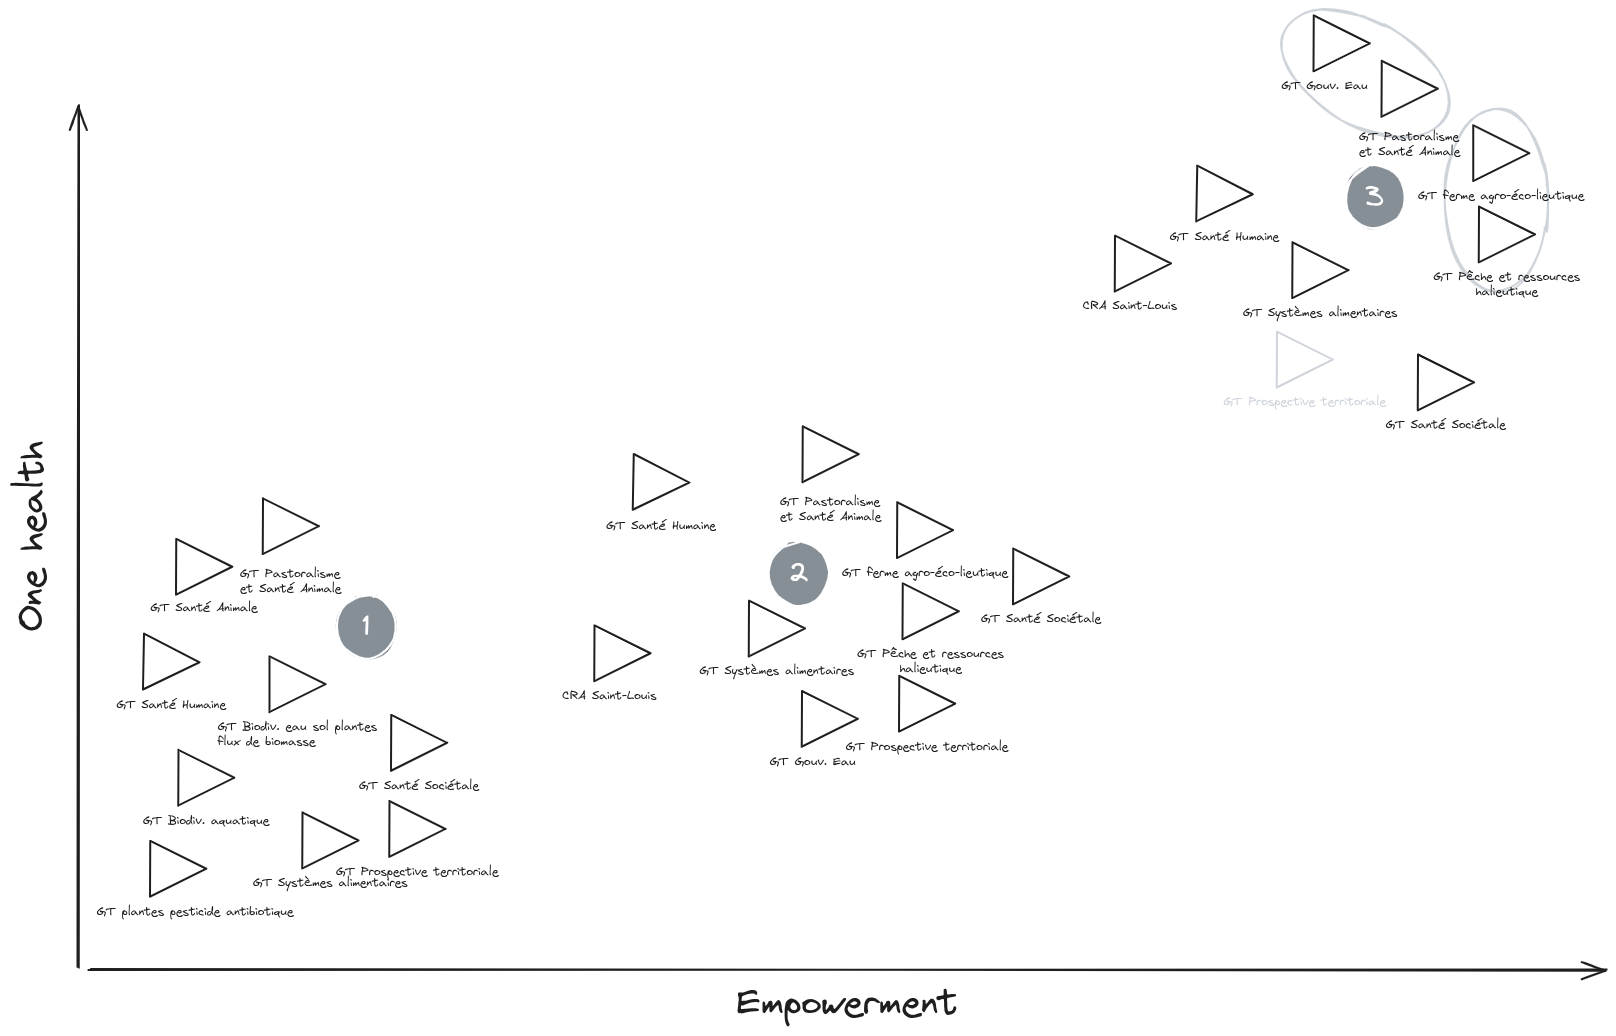
\includegraphics[width=1\linewidth]{img/Drawing 2025-09-07 11.03.30.excalidraw.png}
    \caption{Assemblage of the different groups led by project scientists across the three phases, according to their engagement with the One Health objective and the emancipation of actors. Rearrangements and convergences among groups can be observed over time.}
    \label{fig:alignement-proj}
\end{figure}

Across the three phases we identified—disjointed elements, first convergences, and assemblage in action—the framework of assemblages allows us to read less a “linear progression” than a succession of reconfigurations in which humans, non-humans, rules, and \textit{dispositifs} couple in different ways. First within thematic groups, and once these groups had matured, between thematic groups (see Fig.~\ref{fig:alignement-proj}).  

In line with work that conceives assemblages as socio-ecological and material compositions \parencite{hertz_knowledge_2025}, our observations show that alignment does not stem merely from a convergence of representations but from a patient work of forging attachments that render certain connections tenable: a monitoring protocol, a fish pond, a collective of herders, a water constraint, an agricultural calendar. Each phase corresponds to a transitional state of assemblages: initially dispersed and competing, then stabilized through shared mediations, and finally enacted on the ground by concrete dispositifs (fodder plots, fish ponds, ComMod workshops) that hold together worlds previously disjointed.  

This reading gains clarity when affective “constitutional moments” are resituated within the grammar of translation set out by \textcite{callon_techno-economic_1990} in the famous case of scallops: problematization, interessement, enrollment, mobilization. Key episodes (the revelation of chemical pollution, conflicts between indigenous and non-indigenous fishers, local desire to experiment with fodder) act as operators of interessement: they consolidate attachments around tangible objects and risks, shift boundaries of interest, and open the possibility of enrollment. In other words, affect functions as a locking mechanism, a relational anchoring (one engages because one feels exposed, concerned, connected) that contributes to the reality and realization of action. Conversely, when affect is absent—participation reduced to mere compliance, indicators without addressees, foresight too remote—interessement remains fragile and assemblages unravel, much like Callon’s aborted attempts when actors no longer recognize the “right” entry point into the problem.  

Finally, situating our results within the inspiration of \textcite{hertz_knowledge_2025} underscores the affective character of assemblages: they are architectures where flows of matter and information (water, biomass, data), institutions (fishing rules, sanitary procedures), and artefacts (serious games, biobanks, ponds) co-evolve, influencing and being influenced by affects. The transition from Phase~2 to Phase~3 is not merely narrative; it corresponds to an enhanced capacity for circularity (of knowledge, nutrients, farmers’ or fishers’ incomes influencing well-being) and to strengthened linkages—when a single \textit{dispositif} (for example, fish farming) becomes a pivot simultaneously for nutrition, fisheries regeneration, conflict management among fishers, and water governance. It is precisely here that affect participates in assemblage: dispositifs that make shared benefits and vulnerabilities felt are those that endure and durably reconfigure alliances. This articulation explains why certain convergences (pastoralism–agroecology, fisheries–agro-aquaculture farm) have been reinforced, while others (labeled “One Health” but poorly equipped) remained at a merely declarative stage.  

\subsection{Participation as a Plural and Contested Watchword}

In the project’s documents, participation appears as a consensual watchword: everyone claims it, yet without always designating the same thing. This polysemy is not new; \textcite{arnstein_ladder_1969} already showed that the call to “involve” can cover very different positions, ranging from symbolic manipulation to genuine delegation of power. In our case, this diversity is evident: participation reduced to consultation in some groups (e.g., biomedical data collection), pedagogical participation in others (e.g., veterinary training), and more advanced deliberative participation in co-modeling approaches. The displayed unanimity thus masks a plurality of participation regimes, whose concrete effects on alignment differ greatly.  

In this perspective, the posture adopted in companion modeling (ComMod) processes \parencite{barreteau_our_2003, barreteau_framework_2010} occupies a distinctive place. Whereas participation may sometimes be limited to validating pre-framed options, ComMod rests on putting representations themselves into discussion, through role-playing games, scenarios, or co-constructed models. Participation is no longer just about “adding a voice,” but about collectively transforming the frames of thought and action \parencite{etienne_modepour_2010}. This methodological openness grants participation both a stabilizing power (by aligning divergent visions around shared rules) and an emancipatory capacity (by enabling local actors to reformulate problems and imagine solutions of their own).  

It is striking to note that when ComMod facilitators adopt this posture—neither prescriptive experts nor mere observers—actors find a genuine space of autonomy. Such was the case with the fishers of Mbane who, faced with the disappearance of fish biomass, blamed Malian fishers operating in the area. The researchers’ “letting go” allowed participants to experiment with new rules, test compromises, and inscribe their experience in the making of the common. Where instrumental participation tends to reinforce dependence on experts, participation as operationalized in ComMod opens a pathway to self-organization and agency. It is precisely in this tension between control and emancipation that the transformative scope of participation is at stake: not a consensual slogan, but a field of practices where modes of engagement determine the robustness and durability of collective assemblages.  

\subsection{Affective Moments as Triggers of Reconfigurations}

The dynamics observed in the Senegalese Living Labs show that alignment among thematic groups does not emerge solely from rational debates or institutional framings. More often, it is moments marked by affective intensity—a shock, a dispute, a revelation—that trigger reconfigurations. The exposure of invisible chemical pollution in the lake water, tensions between indigenous and non-indigenous fishers, or the collective enthusiasm around experimenting with fodder crops all acted as revelations. These episodes functioned as “constitutional moments” in \textcite{jasanoff_constitutional_2011}’s sense: they destabilize habitual frameworks and open a space for redefining priorities. In other words, alliances truly transform when knowledge translates into lived, embodied experience.  

This dimension resonates with recent proposals around “affective knowing” \parencite{hertz_knowledge_2025}: a form of knowledge valued not only for its cognitive content but for its capacity to be felt and to mobilize actors. In our case, affect acted as a catalyst for interessement in Callon’s sense \parencite{callon_techno-economic_1990}, by rendering certain problems concrete and pressing. Where indicators or protocols remained abstract, the shared experience of vulnerability—drinking water contaminated with chemicals, losing fishing income, seeing herds threatened—enabled the durable enrollment of actors. The passage from distant knowledge to situated experience transforms discussion into engagement, and information into collective action.  

The effects of these affective moments, however, extend beyond the instant. They contribute to strengthening the robustness of assemblages by inscribing an emotional and memorial dimension into alliances. In this sense, affect is not incidental but a central operator of stabilization: it gives flesh to dispositifs and nourishes a sense of belonging. At the same time, it carries an element of unpredictability, as affects can also reignite divisions or exacerbate conflicts. This is why methodological accompaniment—and particularly the posture of ComMod facilitators—is crucial: the challenge is to transform these intensities into resources for collective action rather than letting them dissipate or harden. Affective moments thus appear as windows of opportunity, from which competing imaginaries can be negotiated and practices recomposed.  

\subsection{Between Sectorialization and Integration: The Difficult Operationalization of One Health}

The \textit{Santés \& Territoires} project illustrates well the limits of an overly generic use of the term One Health. In its international formulation, the concept aspires to be integrative—bringing together human, animal, and environmental health—yet it often remains a normative banner, invoked rather than embodied. In the practices of the thematic groups, One Health only gained real meaning when it became situated: for example, when it materialized in fodder plots connecting pastoral needs, soil fertility, and human nutrition, or in fish farming linking biodiversity, food incomes, and water governance. In other words, One Health integration becomes operational only in concrete, bounded configurations that directly engage actors.  

This necessity of situating One Health echoes the “Promethean gap” described by \textcite{anders_obsolescence_1956}: the chasm between the power of our concepts or technologies and the capacity of individuals to recognize themselves in them and translate them into their lives. As long as One Health remains an abstract idea carried by international institutions, it stays out of reach for local communities. When this gap is reduced—when the concept touches on vital, felt, and shared concerns—it becomes a driver of action. This is precisely what we observed: the shift from One Health as a slogan to One Health as lived experience occurred through its articulation with concrete issues in the Living Labs of Lake Guiers.  

The reduction of this gap is made possible through alignment processes among groups and through dispositifs that give the concept both affective and material consistency. Alignments do not dissolve sectoral divergences (biomedical, agronomic, socio-ecological), but they create junction points where perspectives meet to become tangible and actionable. One Health must be anchored in situated actions (territories, actors, issues) that orient changes in practices. It should serve as a compass toward improving health in its multiple dimensions. In this sense, operationalizing One Health is less a matter of definition than of situated enactment, where actors can recognize their place and act collectively.  

\subsection{The Role of Researchers: Between Facilitation, Mediation, and Agenda-Setting}

The experience of the \textit{Santés \& Territoires} project invites us to reconsider the role of researchers in participatory dispositifs. Contrary to the ideal of exteriority often claimed in the social and environmental sciences, researchers cannot remain “above” the process. They are embedded in the dynamics they observe and inevitably contribute to shaping them, whether they wish to or not. The literature regularly highlights this tension: for \textcite{laslaz_jalons_2017}, a posture of reflexive withdrawal is still possible, but our activities within the project show that in the context of Living Labs, such a stance quickly becomes untenable. Researchers are solicited as facilitators, mediators, and sometimes even as institutional guarantors. Their role necessarily exceeds that of mere knowledge producers.  

Yet this engagement does not translate into a stabilized or “ideal” position to be occupied. Our observations point instead to a form of negative navigation \parencite{morizot_manieres_2020}: researchers advance by identifying roles they refuse to assume—such as that of the prescriptive expert imposing solutions, the neutral facilitator merely distributing speaking turns, or the institutional actor locking in compromises. This process of avoidance, far from signaling disengagement, constitutes a way of preserving spaces of autonomy for other participants. The researchers’ posture is thus constructed through successive withdrawals, through refusals to occupy certain positions, thereby allowing more open and negotiated configurations to emerge.  

This ambivalent engagement raises a strong ethical and political question: how far should researchers involve themselves in the transformations they accompany? The balance is delicate between the temptation to imprint a direction (at the risk of imposing an agenda) and the desire to withdraw (at the risk of allowing existing power relations to persist). The added value of the ComMod approach lies precisely in this tension: researchers do not dictate solutions, but they create conditions in which actors can emancipate themselves and experiment. Their engagement consists less in finding a once-and-for-all “proper place” than in assuming a mobile, reflexive, and negative posture, where the art of facilitation is learned through the refusal of certain self-evidences.  

\subsection{Temporalities and Scales of Action: Between Foresight and Local Urgencies}

The Living Labs of the \textit{Santés \& Territoires} project reveal a significant gap between heterogeneous temporalities: that of researchers and institutions, paced by multi-annual projects and prospective horizons (2027 for \textit{Santés \& Territoires}), and that of local populations, centered on daily urgencies linked to subsistence, water, livestock, or fishing catches. As \textcite{fassin_raison_2010} has shown, the relationship to time is inseparable from a moral relationship: humanitarian interventions—and, perhaps by extension, scientific interventions when they present themselves as unveiling a crisis—are situated in a constant tension between urgency (relieving here and now) and the future (transforming durably). In our case, the prospective approaches carried by researchers often appeared too distant for local actors, while the responses to urgencies seemed derisory in light of the systemic ambitions displayed.  

This temporal tension can also be read through \textcite{fassin_science_2009}’s reactivation of Walzer’s metaphor: some scientists remain “in the cave,” immersed in action and its contradictions, while others seek to maintain a position above the cave, claiming to see the scene in its entirety. The \textit{Santés \& Territoires} project illustrates the ambivalence of these postures. Researchers engaged in participatory workshops experienced conflicts and affects at the same rhythm as local communities, while other academic or institutional actors, more distant, framed the project from long-term horizons (2040 foresight, global One Health scenarios). For the project’s researchers, the ideal position would be to remain at the threshold of the cave: not too distant so as not to propose out-of-touch solutions in a paralyzing critical stance, nor too immersed so as not to lose sight of the broader scene. The articulation between these postures is delicate: too much immersion obscures the overall picture, too much distance detaches from lived realities.  

Finally, \textcite{virilio_fin_2023}’s critique of planning temporality also illuminates our material. For him, modern speed tends to crush long timeframes and privilege the instantaneous, at the risk of disarticulating processes of transformation. In the Living Labs, this critique takes form: the logic of donor-funded projects imposes a rapid calendar, deliverables to enable “disbursement,” oriented toward outputs, while the alignments observed among actors are constructed over a much slower time, built from trials, affects, and experiments. Institutional and financial speed thus enters into contradiction with the relational and ecological temporality required for the operationalization of One Health. The sustainability of constructed assemblages depends on the capacity to negotiate these discordant temporal regimes—urgency, slowness, foresight.  

\subsection{Toward Systemic Transformation: Lessons from the Senegalese Case}

One of the salient results of the \textit{Santés \& Territoires} project is that all actors engaged in the process benefited, to varying degrees, from a form of collective aspiration. Researchers, technicians, elected officials, farmers, and herders all found in the Living Labs an arena for broadening their horizons and engaging with other ways of thinking and acting. Even if this dynamic did not always produce perfect alignment, it enabled mutual learning: biomedical researchers became familiar with agroecological concerns, agricultural practitioners discovered health logics, and local actors gained reference points for grasping the complexity of the One Health concept. In other words, the process generated shared cognitive capital, a first condition for envisioning systemic transformations.  

However, this collective capacity-building faces persistent difficulties when it comes to translating conceptual appropriation into genuine emancipation. Local populations in both Living Labs used participatory tools to articulate their own priorities and negotiate tailored solutions. Yet, on the side of certain research institutions, relinquishing control over scientific agendas remains more problematic. Allowing space for non-academic actors, accepting that their knowledge can redefine research questions, remains a difficult exercise. These hesitations reflect a structural tension: the will to promote transdisciplinary, participatory science, while simultaneously maintaining academic legitimization logics and scientific productivism.  

This observation calls for a nuanced assessment of the model’s reach. The Senegalese case shows that systemic transformation is not merely a matter of tools or methodologies, but of power relations, affects, and recognition. The shared language around One Health undeniably fostered rapprochements and provided a common vocabulary, but its effectiveness rests on institutions’ willingness to accept a redistribution of roles. If researchers remain too inclined to frame trajectories, the emancipation of local participants will remain partial. Conversely, whenever an open space for negotiation was made possible—as in fodder or fish farming experiments—alignments produced tangible and lasting effects. This is perhaps the strongest lesson: for Living Labs to become true engines of systemic transformation, it is not enough to align representations; it is also necessary to redistribute capacities to act, thereby expanding freedoms \parencite{sen_development_1999}. 

\section{Conclusion}

The study of the \textit{Santés \& Territoires} project in Senegal highlights a process of progressive alignment, marked by phases of initial dispersion, uncertain convergences, and eventually stabilized assemblages. This non-linear trajectory was shaped by encounters, tensions, and at times conflicts, but also by shared affective experiences that opened new possibilities (such as the disappearance of fish stocks or the detection of chemical pollutants in water). This dynamic confirms the fertility of the assemblage approach for analyzing transformation projects in their relational and situated dimensions. It allows us to understand how heterogeneous elements—human and non-human, scientific knowledge and local practices, institutions and affects—can coordinate in configurations that make action possible.  

Read through the lens proposed by \textcite{anders_obsolescence_1956}, this analysis also acquires a philosophical resonance. Anders emphasized the “Promethean gap” between the power of our concepts or technologies and the ability of individuals to recognize themselves in them and translate them into their lives. Our results suggest that the assemblage perspective and the sociology of translation offer a concrete way to reduce this gap: by situating global concepts such as One Health in local material and affective dispositifs, they facilitate the passage to transformative action. Far from remaining slogans or promises, these notions become operational once they are embodied in situated practices and mobilize actors through lived experience. In the process, participants gain in agency and thus in freedom \parencite{sen_development_1999}.  

Finally, this study confirms the importance of co-constructing imaginaries. As \textcite{castoriadis_domaines_1999, beckert_uncertain_2018} remind us, in a world of radical uncertainty, it is collectively shared narratives, models, and fictions that orient decisions and coordinate action. When imposed from above or monopolized by a few dominant actors, such narratives risk excluding and freezing possibilities. By contrast, participatory approaches and companion modeling dispositifs make it possible to produce models with stakeholders, rather than for them. These co-constructed models shape the future more equitably and sustainably, redistributing the capacities to imagine, to speak, and to act. In this sense, the Senegalese experience is not merely a local case: it sheds light on the conditions under which transdisciplinary projects can become genuine laboratories of systemic transformation—spaces where knowledge, affects, and shared commitments converge.  


\printbibliography

\end{document}